\documentclass[twocolumn]{aastex63}
\usepackage{natbib}
%\definecolor{orcidlogocol}{HTML}{A6CE39}
\bibliographystyle{aasjournal}

\begin{document}

\title{COLLISION RATES OF PLANETESIMALS NEAR MEAN-MOTION RESONANCES}

\author{Spencer C. Wallace}
\affiliation{Astronomy Department, University of Washington, Seattle, WA 98195}

\author{Thomas R. Quinn}
\affiliation{Astronomy Department, University of Washington, Seattle, WA 98195}

\author{Aaron C. Boley}
\affiliation{Department of Physics and Astronomy, University of British Columbia, Vancouver BC, Canada}

\begin{abstract}
In circumstellar disks, collisional grinding of planetesimals produces second-generation dust which can be observed through thermal 
emission. While it remains unclear when second-generation dust first becomes a major component of the total dust content, the presence of 
such dust and potentially the substructure within it can be used to explore a disk's physical conditions. A perturbing planet has been shown to 
produce nonaxisymmetric structures, as well as gaps in disks, regardless of the origin of the dust. However, small grains will have very 
different dynamics compared with planetesimals when in the presence of gas, and as such, the collisional evolution of planetesimals could 
create dusty disk structures that would not exist otherwise. Previous studies have shown that morphological differences in the collisional dust 
corotating with a giant planet can be used to determine whether the planet's eccentricity is large or small. Going further, we investigate the 
production of second-generation dust near prominent mean-motion resonances with the planet using N-body simulations that directly resolve 
collisions between planetesimals. We find that a distinct over- or under-density in the dust emission is produced at the interior 2:1 mean motion 
resonance, depending on the mass and eccentricity of the planet. The presence of one of these two features can be used to place simultaneous 
upper or lower limits on the mass and eccentricity of the perturbing body.
\end{abstract}

\section{Introduction} \label{sec:intro}

Recent observations of circumstellar disks by ALMA have revealed a rich variety of substructure in the millimeter contiunuum emission. Features 
such as gaps and asymmetries 
\citep{2015ApJ...808L...3A, 2016Sci...353.1519P, PhysRevLett.117.251101, 2016ApJ...820L..40A, 2016Natur.535..258C} in the emission provide 
diagnostics for the physical processes that drive the evolution of the disks. In some cases, these gap features are argued to be an indicator for the 
presence of a giant planet, either embedded in the disk \citep{2015MNRAS.453L..73D} or orbiting externally. A giant perturber can influence the 
structure of the continuum emission in a number of ways. A misaligned giant planet can produce nonaxisymmetric features such as warps 
\citep{2001A&A...370..447A}. Highly eccentric perturbers can produce even more complicated structures through secular perturbations 
\citep{2014MNRAS.443.2541P, 2015MNRAS.448.3679P}. Mean motion resonances (MMRs) have been shown to open gaps as well 
\citep{2015ApJ...798...83N, 2016ApJ...818..159T, 2018ApJ...857....3T}.

Collisions between planetesimals are thought to be a significant source of dust for many young circumstellar disks 
\citep[see][]{2008ARA&A..46..339W}. An expanding debris cloud from a planetesimal collision was recently detected through scattered light in the 
Fomalhut system \citep{2020PNAS..117.9712G}. Although some amount of primordial dust is likely still present during the planet formation process, 
ongoing collisions between small bodies will augment this and could be used to trace the underlying dynamical activity of the planetesimals. 
\citet{2013ApJ...777L..31D} showed that collisional dust generated near the gap formed by a giant planet in a planetesimal disk should produce a 
distinctly observable marker that could be used to infer the presence of the planet. In a followup study, it was found that morphological differences in 
the dust emission could be used to distinguish between a low and high eccentricity planet \citep{2016ApJ...820...29D}.

Although more difficult to spatially resolve, substructure due to mean-motion resonances (MMRs) with a giant planet may hold additional clues which 
could be used to constrain the properties of the planet.  The width of a resonance is set by both the mass of the perturbing planet, along with the 
unperturbed eccentricity of the planetesimals, which is in turn set by the eccentricity of the planet through secular forcing. Therefore, the structure of 
second generation dust produced near MMRs may hold information about both the mass and eccentricity of the planet.

The dynamics governing the motion of bodies near MMRs is extremely nonlinear, as is determining what the collision rates between planetesimals 
should look like in these regions. For a collection of bodies massive enough to experience the effects of gravitational focusing, a large eccentricity 
dispersion tends to reduce the probability of collision, while enhancements in surface density tends to increase it. Due to conservation of the Jacobi 
energy, MMRs simultaneously enhance the local eccentricity dispersion and also enhance the surface density adjacent to the resonance 
\citep{2000Icar..143...45R, 2017ApJ...850..103B}. Unfortunately, collision detection in an N-body simulation is extremely computationally expensive. 
So far, studies of planetesimal dynamics near MMRs have involved either collisionless test particles 
\citep{2017ApJ...850..103B, 2016ApJ...818..159T, 2018ApJ...857....3T} or severely limited integration times \citep{2000Icar..143...45R}.

To further elucidate this subject, we use the tree based N-body code {\sc ChaNGa}
\citep{2008IEEEpds...ChaNGa, 2015AphCom..2..1} to follow the collisional evolution of a planetesimal disk under the gravitational 
influence of a Jupiter sized body. Because particle positions are sorted into a tree structure, neighbor finding and collision detection 
can be done quickly and efficiently. This considerably relaxes the constraints on resolution and integration time. With this toolset, we 
explore the collision rate structure of the planetesimal disk in the vicinity of mean motion resonances. In particular, we would like to 
determine: 1. whether MMRs leave a detectable signature in the collisionally-generated dust. 2. If these signatures can be used to determine or 
constrain the orbital properties of the perturbing planet.

This work is organized in the following way: In section \ref{sec:dynamics}, we provide an overview of the relevant dynamics that drive the evolution 
of a planetesimal disk under the gravitational influence of an external perturber. In section \ref{sec:sims} we provide an overview of the N-body code 
that we use and describe the initial conditions that are used for five simulations in which a perturbing giant planet is given is given various masses 
and eccentricities. Section \ref{sec:results} presents the results of these five simulations and we use the collision statistics to generate synthetic dust 
emission profiles that would be detected with observing facilities like ALMA. Next, we show in section \ref{sec:constrain} that a characteristic bump 
or dip feature appears in the dust emission near the interior 2:1 MMR, the presence of which depends on the mass and eccentricity of the perturbing 
planet. We discuss the potential of using this feature to place and upper or lower on the mass and eccentricity of the planet and conclude in section 
\ref{sec:conclusions}.

\section{Overview of Relevant Dynamics} \label{sec:dynamics}

\subsection{Secular Forcing}\label{sec:sec_force}

The most direct and widespread effect that a giant perturber will have on a planetesimal disk is through secular forcing of the 
eccentricities of the planetesimals. This will cause the complex eccentricities of the planetesimals to take on a time independent 
forced value, given by \citep{1999ApJ...527..918W} as

\begin{equation}\label{eq:eforced}
	z_{f} = \frac{b^{2}_{3/2} (\alpha)}{b^{1}_{3/2} (\alpha)} e_{g} ~ \mathrm{exp} ~ i \omega_{g}.
\end{equation}

\noindent Here, $\alpha = a_{g} / a$ where $a_{g}$ and $a$ are the semi-major axes of the giant planet and the planetesimal, 
respectively. $e_{g}$ and $\omega_{g}$ are the eccentricity and longitude of pericenter of the giant and $b^{j}_{s} (\alpha)$ is a 
Laplace coefficient given by \citep{2000ssd..book.....M} as

\begin{equation}\label{eq:lap}
	b_{s}^{j}(\alpha) = \frac{1}{2 \pi} \int_{0}^{2 \pi} \frac{cos \, j \theta \, d \theta}{\left( 1 - 2 \alpha \, cos \theta + \alpha^2 \right)^{s}}.
\end{equation}

Without any nearby secular or mean motion resonances, equation \ref{eq:eforced} will completely describe the eccentricities and longitude of  
pericenter orientations of the planetesimals. Additional forces due to two-body scattering between planetesimals, along with 
aerodynamic gas drag will add an additional free component to the complex eccentricity, which will be randomly oriented. The 
magnitude of the free eccentricity describes how dynamically hot the planetesimal disk is and sets the random encounter speeds of 
planetesimals. When the dynamical excitation of the disk is driven by gravitational stirring, the magnitude of the free eccentricity can 
be described by a Rayleigh distribution \citep{1992Icar...96..107I}.

\subsection{Mean Motion Resonances}

In regions where there are commensurabilities between frequencies, secular theory breaks down and bodies are subject to strong 
perturbations. For the purposes of this study, we will ignore secular resonances, which generally occur on rather large timescales 
and will focus on mean motion resonances (MMRs). A MMR occurs  when the orbital period ratio between two bodies is sufficiently 
close to

\begin{equation}\label{eq:per_mmr}
	\frac{P}{P'} = \frac{p + q}{p},
\end{equation}

\noindent where  $p$ and $q$ are integers $>$ 0 and the unprimed and primed quantities correspond to the perturber and the body 
being perturbed, respectively. If the perturber is much more massive than the other body, the condition for MMR is set  by the semi-major 
axes of the two bodies by

\begin{equation}\label{eq:a_mmr}
	\frac{a}{a'} = \left( \frac{p}{p + q} \right)^{2/3}.
\end{equation}

If we further assume that the two bodies are orbiting in the same plane, the behavior of the bodies near resonance is determined by the
behavior of a critical angle

\begin{equation}\label{eq:phi_crit}
	\phi = (p + q) \lambda' - q \lambda - (2 p + q) \varpi,
\end{equation}

\noindent where $\lambda = \varpi + M$ is the mean longitude of a body. For bodies in resonance, the critical angle will librate around an 
equlibrium value, while this angle will circulate outside of resonance. This behavior is analogous to the motion of a pendulum. Changes in the 
critical angle are coupled to changes in the mean motion and semimajor axis \citet{2000ssd..book.....M}. An important point to note, which will 
become important later, is that the circulation frequency approaches zero near the edge of a resonance. The width of a resonance can be 
defined by determining the largest variation in semimajor axis that permits librational, rather than circulatory motion of the pendulum. For 
second and higher order resonances, the maximum libration width is given by

\begin{equation}\label{eq:res_so}
	\frac{\delta a}{a} = \pm \left( \frac{16}{3} \frac{\left| C_{r} \right|}{n} e^{\left| 2 p + q \right|} \right)^{1/2},
\end{equation}

\noindent where n, a and e are the mean motion, semimajor axis and eccentricity of the unperturbed body. $C_{r}$ is a constant defined by 
$m'/m_{c} n \alpha f_{d}(\alpha)$, where $\alpha$ = $a/a'$ and $f_{d}$ is the resonant part of the disturbing function. For an interior second-order 
resonance,

\begin{equation}\label{eq:fd_so}
	f_{d} (\alpha) = \frac{1}{8} \left[ -5(p+q) + 4(p+q)^{2} - 2 \alpha D + 4(p+q) \alpha D + \alpha^{2} D^{2} \right] b^{p+q}_{1/2},
\end{equation}

\noindent where $D b^{j}_{s}$ is the first derivative with respect to $\alpha$ of the Laplace coefficient defined in equation \ref{eq:lap}. This can 
be written as

\begin{equation}\label{eq:lap_d}
	\frac{d b_{s}^{j}}{d \alpha} = s \left( b_{s+1}^{j-1} - 2 \alpha b_{s+1}^{j} + b_{s+1}^{j+1} \right).
\end{equation}

For a first order resonance, the associated disturbing function terms are slightly simpler

\begin{equation}\label{eq:fd_fo}
	f_{d}(\alpha) = (p+q) b_{1/2}^{p+q} + \frac{\alpha}{2} D b_{1/2}^{p+q},
\end{equation}

\noindent and there is an additional contribution to the motion of the critical angle by the pericenter precession rate such that

\begin{equation}\label{eq:res_fo}
	\frac{\delta a}{a} = \pm \left(\frac{16}{3} \frac{\left| C_{r} \right|}{n} e \right)^{1/2} \left(  1 + \frac{1}{27 p^2 e^3} \frac{\left| C_{r} \right|}{n} 
	\right)^{1/2} - \frac{2}{9 p e}  \frac{\left| C_{r} \right|}{n}.
\end{equation}

Changes in eccentricity are correlated with changes in semimajor axis variations according to the Tisserand relation

\begin{equation}\label{eq:tiss}
	\frac{de}{da} = \frac{a^{3/2} - 1}{2 a^{5/2} e}.
\end{equation}

The net result of this is that MMRs will produce 'spikes' in the semimajor axis - eccentricity distribution of a planetesimal disk. In order to 
preserve the Jacobi energy, equation \ref{eq:tiss} predicts that these spikes will tend to curve away from the perturbing body. This lowers the 
surface density of the disk near the locations of resonances, while producing a pileup of bodies on eccentric orbits adjacent to the MMR. The 
enhanced surface density will increase the collision rate. At the same time, the large eccentricites will either lower it due to the decreased 
effectiveness of gravitational focusing, or raise it due to the more vigorous encounter rate, depending on how large the encounter velocity gets 
compared to the escape velocity of the planetesimals. In addition, the MMRs cause the orbits of planetesimals to precess on relatively short 
timescales, which effectively randomizes their longitudes of perihelion. In a secularly forced disk, there will be an interface between aligned 
and randomly oriented orbits at the edge of the resonance. Due to the complicated dynamics that are at play in this region, we turn to a direct 
N-body treatment to better understand how the collision rate varies in the vicinity of a MMR.

\section{Simulations} \label{sec:sims}

\subsection{Numerical Methods}\label{sec:methods}

To follow the dynamical and collisional evolution of a planetesimal disk, we use the highly parallel N-body code {\sc ChaNGa} 
\footnote{A public version of {\sc ChaNGa} can be downloaded from \url{http://www-hpcc.astro.washington.edu/tools/ChaNGa.html}}. 
This code, which is written in the {\sc CHARM++} parallel programming language, was originally designed for cosmology simulations 
and has been shown to perform well on up to half a million processors \citep{2015AphCom..2..1}. {\sc ChaNGa} calculates 
gravitational forces using a modified Barnes-Hut \citep{1986Natur.324..446B} tree with hexadecapole expansions of the moments. 
All of the simulations we perform use a node opening criterion of $\theta_{BH}$ = 0.7. More information about the code can be found 
in \citet{2008IEEEpds...ChaNGa}. We have also recently modified {\sc ChaNGa} to handle solid-body collisions. A full description of 
the collision module implementation can be found in \citet{2019MNRAS.489.2159W}.

\begin{table}
\begin{center}
\caption{Summary of Simulations Run}
\begin{tabular}{lllll} \hline \hline
Name     & Mass of Planet & Eccentricity of Planet &  &  \\ \hline
e1m2 & 1.0 $M_{jup}$                     & 0.5 $e_{jup}$                            &  &  \\
e2m2      & 1.0 $M_{jup}$                     & 1.0 $e_{jup}$                             &  &  \\
e3m2 & 1.0 $M_{jup}$                     & 2.0 $e_{jup}$                             &  &  \\
e2m1 & 0.5 $M_{jup}$                   & 1.0 $e_{jup}$                             &  &  \\
e2m3 & 2.0 $M_{jup}$                     & 1.0 $e_{jup}$                             &  &  \\ \hline
\end{tabular}
\label{tab:sims}
\end{center}
\end{table}

\subsection{Initial Conditions}\label{sec:ics}

In total, five simulations are run. The first is a 'nominal' case, in which the perturbing planet's mass and eccentricity are set to that of Jupiter's. 
In the other four cases, the mass (eccentricity) is increased or decreased by a factor of two, while the mass (eccentricity) is held at the nominal 
value. In all cases, the perturbing giant is placed on a 5.2 AU orbit around a 1 $M_{\odot}$ star. The planetesimal disk extends from 2.2 to 3.8 
AU, which covers the two most prominent mean motion resonances with the giant planet, the 2:1 at 3.27 AU and the 3:1 at 2.5 AU.The 
planetesimal disk follows a minimum-mass solar nebula surface density profile \citep{1981PThPS..70...35H}

\begin{equation}\label{eq:surf_den}
	\Sigma = \Sigma_{0} r^{-\alpha},
\end{equation}

\noindent with $\alpha$ = 3/2 and $\Sigma_{0}$ = 10 g cm$^{-2}$. Planetesimals are given a bulk density of 2 g cm$^{-3}$ and a diameter of 
300 km. This corresponds to a disk containing roughly 500,000 bodies. Each simulation is evolved for 5,000 years, which is about 400 Jupiter 
orbits.

The dynamical effects of secular forcing by the giant planet, along with  the effects of viscous stirring and gas drag on the planetesimals, are 
built into the initial conditions. This is done by first calculating the equilibirum eccentricity $e_{eq}$ due to viscous stirring and gas drag as a 
function of semimajor axis according to equation 12 of \citet{2002ApJ...581..666K}. Although {\sc ChaNGa} does not account for the effects of 
gas drag on the planetesimals, the viscous stirring timescale is long compared to our integration time and should not cause the velocity 
distribution to significantly evolve. The eccentricities of the bodies are drawn randomly from a Rayleigh distribution with a mode of $e_{eq}$, 
while the inclinations are drawn from a similar distribution with a mode of $e_{eq}$/2 \citep{1993MNRAS.263..875I}. The longitude of perihelia 
$\omega$ and the mean anomalies $M$ of the bodies are drawn from a uniform polar distribution.

To account for the effects of secular forcing, the eccentricity vectors of the planetesimals are first decomposed into real and imaginary 
components:

\begin{equation}\label{eq:hk}
	z = (h, ik) = e \, exp(i \omega)
\end{equation}

\noindent and a forced component is added to $h$ according to equation \ref{eq:eforced} (where we have set $\omega_{g}$ = 0).

\subsection{Time Stepping Scheme}\label{sec:timestep}

For the purposes of the integrator, there are two relevant timescales in this system. The first is the orbital dynamical time $\sqrt{a^3/
G M_{\odot}}$. All particles are placed on a fixed time step of $\Delta T$ = 0.01 yr. This is roughly 3\% of an orbital dynamical time at 
the inner edge of the planetesimal disk. From numerical tests with {\sc ChaNGa}, we have found that this time step size preserves 
the symplectic nature of the integration without being too computationally expensive. Although using $\Delta T$ = 0.01 yr keeps the 
integration symplectic, we find that a small amount of artificial precession is produced. We reduce the base time step size by an additional 
factor of 4 to the keep longitude of perihelia of planetesimals near the inner edge of the disk from drifting too far over the course of our 
integrations.

An additional timescale is set by the dynamical time of the planetesimals ($\sim 1/\sqrt{G \rho}$), which is about 45 minutes. To 
resolve the base time step and the dynamical timescale of planetesimals simultaneously, we use a two-tiered time stepping scheme. 
To start, all bodies are placed on the orbital time step. A first pass of collision detection is then run in 
which the radii of all bodies are inflated by a factor of 2.5. Any bodies with imminent collisions predicted using the inflated radii are 
placed on a time step that is a factor of 16 smaller than the orbital time step. The purpose of two-tiered scheme is to properly resolve 
the gravitational interactions between any bodies that undergo a close encounter. This prevents the coarser base time step from 
reducing the effectiveness of gravitational focusing, while minimizing the additional computational expense.

\begin{figure*}
\begin{center}
    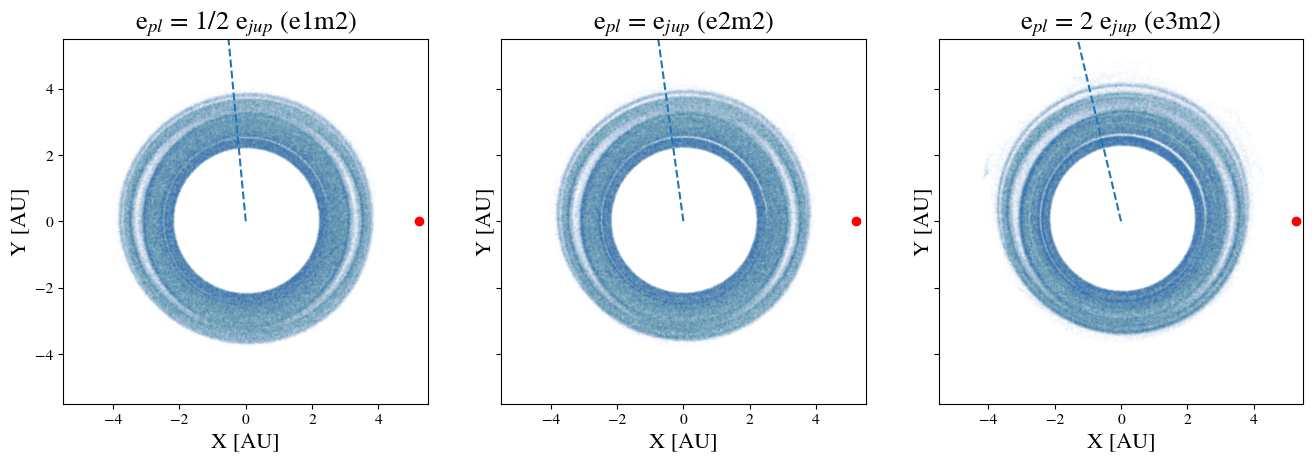
\includegraphics[width=\textwidth]{figures/xy.png}
    \caption{The positions of the remaining planetesimals at the end of the e1m2 (left), e2m2 (center) and e3m2 (right) simulations. The red dot 
    indicates the position of the giant planet and the dashed line points in the direction of the planet's longitude of perihelion. Non-axisymmetric gaps 
    are apparent near the locations of MMRs. At higher eccentricities, more resonances become visible. At the 2:1 MMR, gap features at $\theta$ = 0 
    and $\theta = \pi$ follow the giant planet in its orbit.\label{fig:xy}}
\end{center}
\end{figure*}

\begin{figure}
\begin{center}
    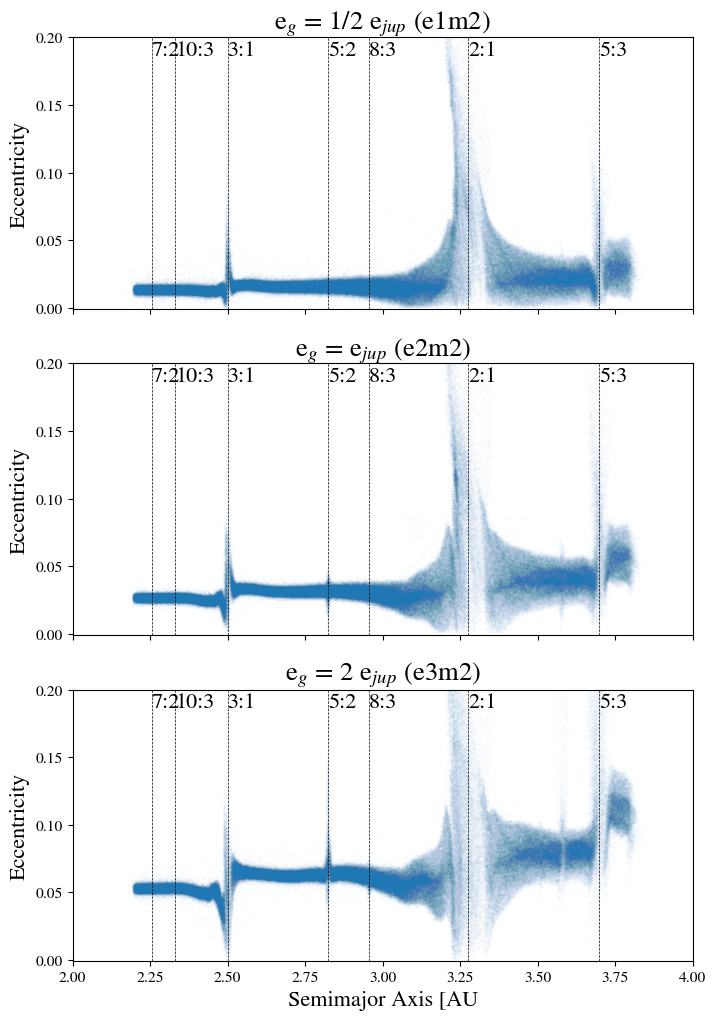
\includegraphics[width=0.5\textwidth]{figures/ae.png}
    \caption{The semimajor axes and eccentricities of the remaining planetesimals are shown, with the locations of prominent resonances indicated 
    by the vertical dashed lines. Libration of the critical angle drives large variations in eccentricity, which produce spikes in the a-e plane. Between 
    the resonances, the nonzero eccentricity is due to secular forcing by the planet.\label{fig:ae}}
\end{center}
\end{figure}

\begin{figure*}
\begin{center}
    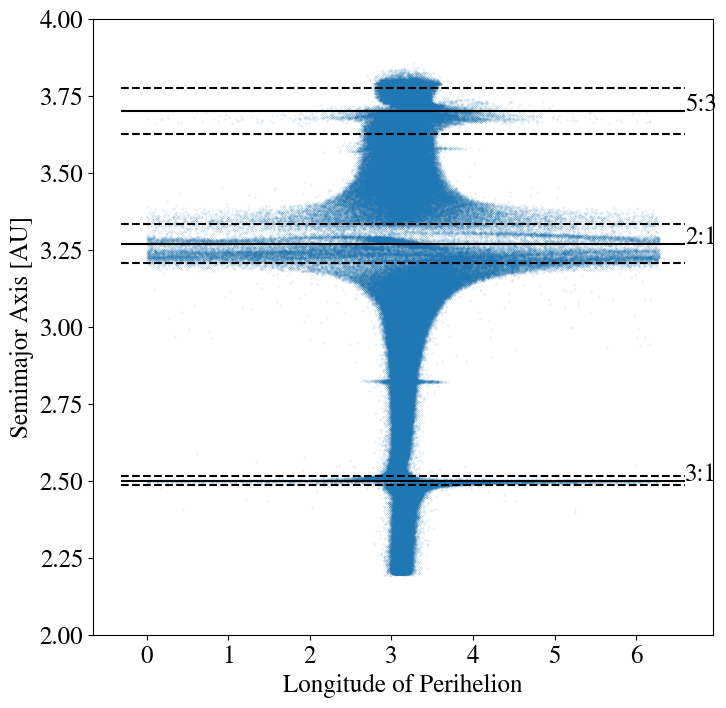
\includegraphics[width=\textwidth]{figures/long_ph.png}
    \caption{Shown here are the longitudes of pericenter and semimajor axes of the remaining planetesimals. The dashed lines again indicate the 
    locations of prominent MMRs. Close to the resonances, the critical angle librates and drives fast precession of the longitudes of pericenter of the 
    bodies. This overpowers the secular forcing by the planet and effectively randomizes the orientations of their orbits.\label{fig:long_ph}}
\end{center}
\end{figure*}

\section{Results} \label{sec:results}

All five simulations are evolved for 5,000 years, which is roughly 400 orbits of the perturbing planet. Because the effects of the mean motion 
resonances are not built into the initial conditions, the simulations must be run long enough for the distribution of orbital elements to reach 
equilibrium near the resonances before the collision rate is measured. The libration timescale, which describes how long the critical angle (and also 
the semimajor axis and eccentricity) of a planetesimal in resonance takes to undergo a full oscillation is given by

\begin{equation}\label{eq:lib_time}
	T_{lib} = \frac{2 \pi}{3 q^{2} C_{r} n e^{\left| 2p + q \right|}},
\end{equation}

\noindent for small-amplitude librations. For all five sets of initial conditions used, $T_{lib} \sim$ 1,000 - 2,000 years for the 3:1 and 2:1 resonances. 
For this reason, we allow each simulation to run for 2,000 years before we begin tracking any collision statistics.

\subsection{Varying the Eccentricity}

We begin by examining simulations e1m2, e2m2 and e3m2. The positions of the planetesimals in the x-y plane after 5,000 years of integration is 
shown in figure \ref{fig:xy}. In all cases, the coordinate system is rotated so that the giant planet lies at $\theta = 0$ and the longitude of perihelion of 
the planet is shown by the dashed line. Resonances with the perturbing planet are visible via nonaxisymmetric gaps. Upon close inspection of the 
last few simulation snapshots, these gaps appear to follow the planet in its orbit, rather than aligning themselves with the longitude of perihelion. A 
similar substructure reveals itself in \citet{2000Icar..143...45R} (see bottom panel of figure 3) and \citet{2016ApJ...818..159T} (figure 3). It is worth 
noting that \citet{2000Icar..143...45R} started with a completely cold planetesimal disk and a Jupiter mass planet on a circular, coplanar orbit. The 
presence of these features seems robust to the choice of initial conditions.

The effects of the resonances become much more apparent in semimajor axis-eccentricity space, which is shown in figure \ref{fig:ae}. In all cases, 
the 3:1, 2:1 and 5:3 resonances are readily visible as 'spikes' in the eccentricity that bend slightly inward (due to the conservation of $E_{J}$). In the 
e3m2 simulation, features also appear near the 5:2, 7:3 and 5:3 resonances. The absence of these features from the e1m2 simulation can be 
explained by the fact that the strength of a resonance scales with $e^{q}$ \citep{1994PhyD...77..289M}.

Another important effect of the resonances is visible in figure \ref{fig:long_ph}, which shows the orientation of the longitude of perihelia of 
planetesimals in the disk. Inside of the resonances, orbits of planetesimals quickly precess and their orientations are effectively randomized. An 
important point to note is that this strong precession effect quickly disappears beyond the boundaries of the resonance. This turns out to be 
important to explain the nonaxisymmetric structure seen in figure \ref{fig:xy}, which will be addressed in more detail below.

Next, we examine the statistics of collisions resolved in each of the simulations. The 3D positions and velocities of the two colliding bodies are 
recorded to a table at the moment of impact. From these quantities, we also derive the Keplerian orbital elements of a collision from these quantities. 
First, we examine the semimajor axis of the first particle participating in each collision. During a collision, the 'first' particle is defined as the more 
massive of the two. However, nearly all of the collisions happen between the initial, equal-mass planetesimals. In this case, the distinction is set by 
the collision search algorithm and is rather arbitrary. In all of the plots where we show collision statistics, we have verified that using the 'first' or 
'second' collider does not qualitatively change any of the features.

Figure \ref{fig:coll_hist_a} shows the semimajor axis distribution of the resolved collisions. We find that some of the features present in this and 
subsequent figures are highly sensitive to the number of bins and the location of the bin edges. For this reason, we construct a PDF of the collisions 
using a Kernel Density Estimate (KDE). We use the {\sc neighbors.KernelDensity} function from the {\sc sklearn} \citep{scikit-learn} package to 
construct our KDEs. For the kernel, we use a tophat function with a bandwidth of 0.02 AU.

Near some of the resonances, there are noticeable suppressions or enhancements of the local collision rate. This contrasts with the findings of 
\citet{2000Icar..143...45R}, who simulated a similar setup and found no discernible features near the MMRs. We attribute the differences to  a more 
conservative timestepping criterion in our simulations. The most prominent features appear as an enhancement to the collision rate near the 2:1 
MMR and a decrease near the 3:1 MMR. At higher forced eccentricities, features near the 5:2, 7:3 and 5:3 resonances are also visible, due to the 
steeper sensitivity of higher order resonances to eccentricity \citep{1994PhyD...77..289M}.

We attribute the production of a bump vs a dip at certain resonances to changes in the gravitational focusing factor during two-body encounters. 
Closer to the star, the planetesimal disk starts off dynamically colder. Here, additional heating from the resonance acts to suppress the gravitational 
focusing cross section, which reduces the collision rate from the non-perturbed value. Further out in the disk, where the encounter velocity is already 
higher, the gravitational focusing cross section is already minimized. Any additional heating instead acts to simply increase the encounter rate 
between bodies, which enhances the collision rate. This explains the relative drop in the collision rate near the 3:1 MMR and the bumps that form 
near the 2:1 and 5:3 resonance. Although this could potentially serve as a useful diagnostic of the planetesimal size in a disk (because the mutual 
escape velocity sets how dynamically hot the bodies can get before gravitational focusing is suppressed), a direct measurement of the semimajor 
axes of the planetesimals is not possible. In addition, as will demonstrate next, collisions due to bodies in resonance end up having an insignificant 
effect on the final shape of the radial dust distribution.

\begin{figure}
\begin{center}
    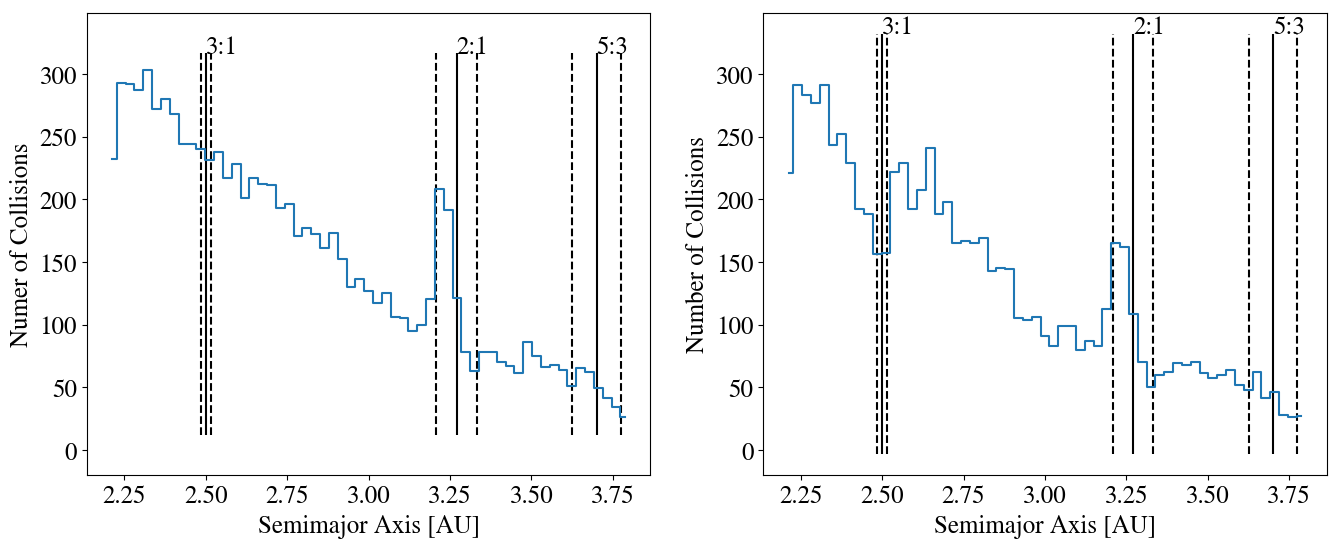
\includegraphics[width=0.5\textwidth]{figures/coll_hist_a.png}
    \caption{In semimajor axis space, prominent features appear near the 3:1 and 2:1 MMRs. Near the 3:1, the collision
    rate decreases from its unperturbed value, while an enhancement apepars near the 2:1.\label{fig:coll_hist_a}}
\end{center}
\end{figure}

\begin{figure}
\begin{center}
    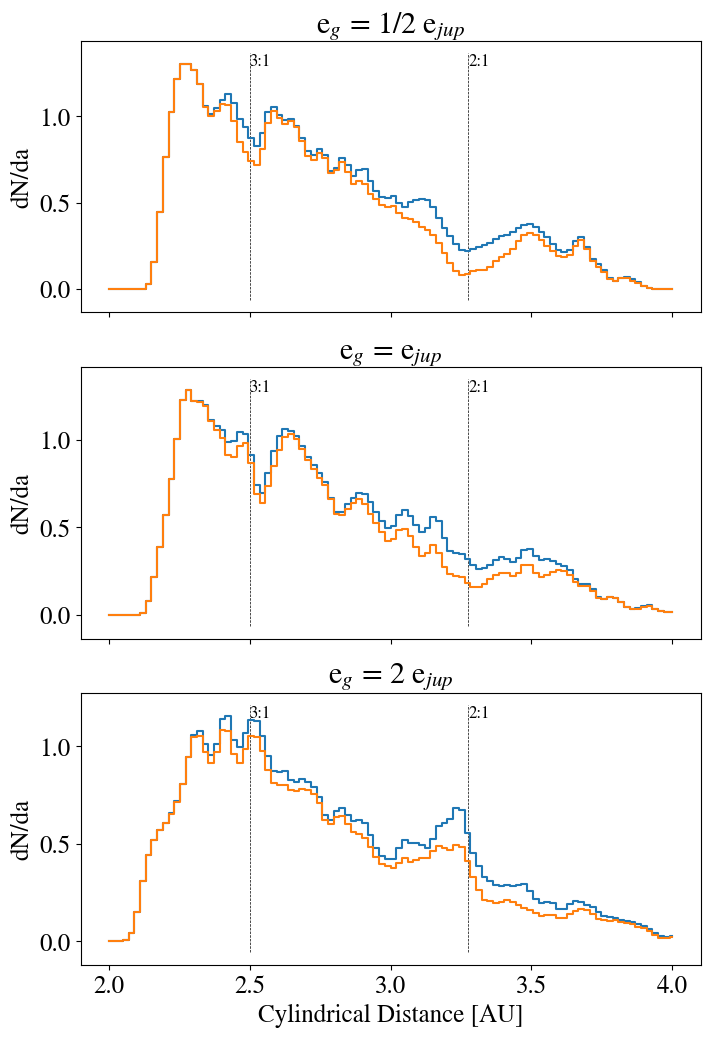
\includegraphics[width=0.5\textwidth]{figures/coll_hist_r.png}
    \caption{Here, collisions are instead ordered by cylindrical distance from the star. Features near the 3:1 and 2:1 MMRs are still present, but appear qualitatively different than in semimajor axis space. At low eccentricities, a dip appears around the center of the resonance. At the highest eccentricity, a bump is formed instead. In orange, the collision profile is shown with collisions between bodies in resonance removed. The bump and dip features remain qualitatively the same, which suggests that they are produced by bodies outside of resonance.\label{fig:coll_hist_r}}
\end{center}
\end{figure}

\subsection{Where Does the Dust End Up?}

To construct a radial dust profile from the collision statistics, we begin by making the assumption that any dust generated by collisions is strongly 
coupled to the gas. For a dust grain larger than the mean free path of the gas particles, the timescale to damp its eccentricity is given by 
\citep{1976PThPh..56.1756A}

\begin{equation}\label{eq:t_edamp}
    t_{e, damp} = \frac{8 s \rho}{3 e C_{D} \rho_{g} v_{th}}.
\end{equation}

\noindent where $m$, $e$ and $s$ are the mass, eccentricity and radius of the dust grain. $C_{D}$ is a drag coefficient which is of order unity, $
\rho_{g}$ is the local density of the gas and $v_{th}$ is its thermal speed. At 3 AU, the gaseous component of the solar nebula has a density of $4 
\times 10^{-10}$ g cm$^{-3}$ and a typical thermal speed of $10^{5}$ cm s$^{-1}$ \citep{1981PThPS..70...35H}. For a 1 mm dust grain with a 
density of 1 g cm$^{-3}$ and an eccentricity of 0.05, the damping timescale is $4 \times 10^{-3}$ years. This is orders of magnitude smaller than the 
collision timescale, therefore we conclude that collisionally generated dust grains will immediately couple to the gas.

Operating under this assumption, a map of the relative concentration of second-generation dust can be constructed from the cylindrical 
distance at which the collisions occur. This is shown in figure \ref{fig:coll_hist_r}. Similar to figure \ref{fig:coll_hist_a}, we use a KDE with a bandwidth 
of 0.02 AU to assemble the collision locations into a radial distribution. Most strikingly, the bump that was present near the 2:1 resonance is no 
longer present in cylindrical distance space, although it suddenly appears again in the e3m2 simulation. The dip that is present near the 3:1 MMR 
also disappears and instead presents as a bump in the e3m2 case. To determine how the resonant bodies actually contribute to the radial collision 
profile, we excluded collisions that fall between $2.495 < a < 2.505$ AU (near the 3:1 resonance) and between $3.2 < a < 3.35$ AU (near the 2:1 
resonance), which is shown by the orange curve. Qualitatively, none of the bump or dip features present are changed by making this exclusion. This 
suggests that the features near resonance seen in semimajor axis space become 'smeared out' in cylindrical distance space due to the large spread 
in eccentricity and orbital orientation.

This also suggests that the features seen in figure \ref{fig:coll_hist_r} are being produced by bodies outside of resonance. To further understand this, 
we revisit the nonaxisymmetric structure seen in figure \ref{fig:xy}. In figure \ref{fig:coll_polar_e}, we compare the radial collision profile to the polar 
structure seen in the e1m2, e2m2 and e3m2 simulations. In the lowest forced eccentricity case, the pileups near the edges of the resonances line up 
with the boundaries of the dip feature seen in the radial collision profile. The locations of the edges of the resonances are calculated using equations 
\ref{eq:res_fo} and \ref{eq:res_so}. The pileups are especially prominent for the 2:1 resonance. As discussed previously, the pileups and gaps seen 
in polar coordinates follow the position of the giant planet in its orbit.

Although the nonaxisymmetric pileup of bodies near the edges of resonances has been seen previously 
\citep{2000Icar..143...45R, 2016ApJ...818..159T}, we could not find a satisfactory explanation for why it happens and will provide one here. As 
mentioned previously, the circulation frequency of the critical angle slows as one approaches the edge of the resonance from the outside. Following 
the pendulum analogy, this is equivalent to reaching the point where the pendulum becomes suspended in the vertical position. When the critical 
angle stays relatively stationary during an encounter, the net torque will drive the longitude of pericenter towards the point of conjunction 
\citep{1976ARA&A..14..215P}.  This is the basic mechanism that causes isolated resonances to be stable. Inside of resonance, the critical angles 
librates about some value and this configuration is maintained. Just outside of resonance, however, the critical angle slowly drifts away, with the drift 
direction changing sign across the resonance. The net result of this is that bodies near the edge of the resonance experience a torque from that 
planet that temporarily drives their pericenters toward the current orbital position of the planet. After the encounter ends, differential rotation of the 
disk slowly destroys the configuration over part of an orbit. This explains why the concentration of planetesimals appears to 'follow' the the planet.

\begin{figure*}
    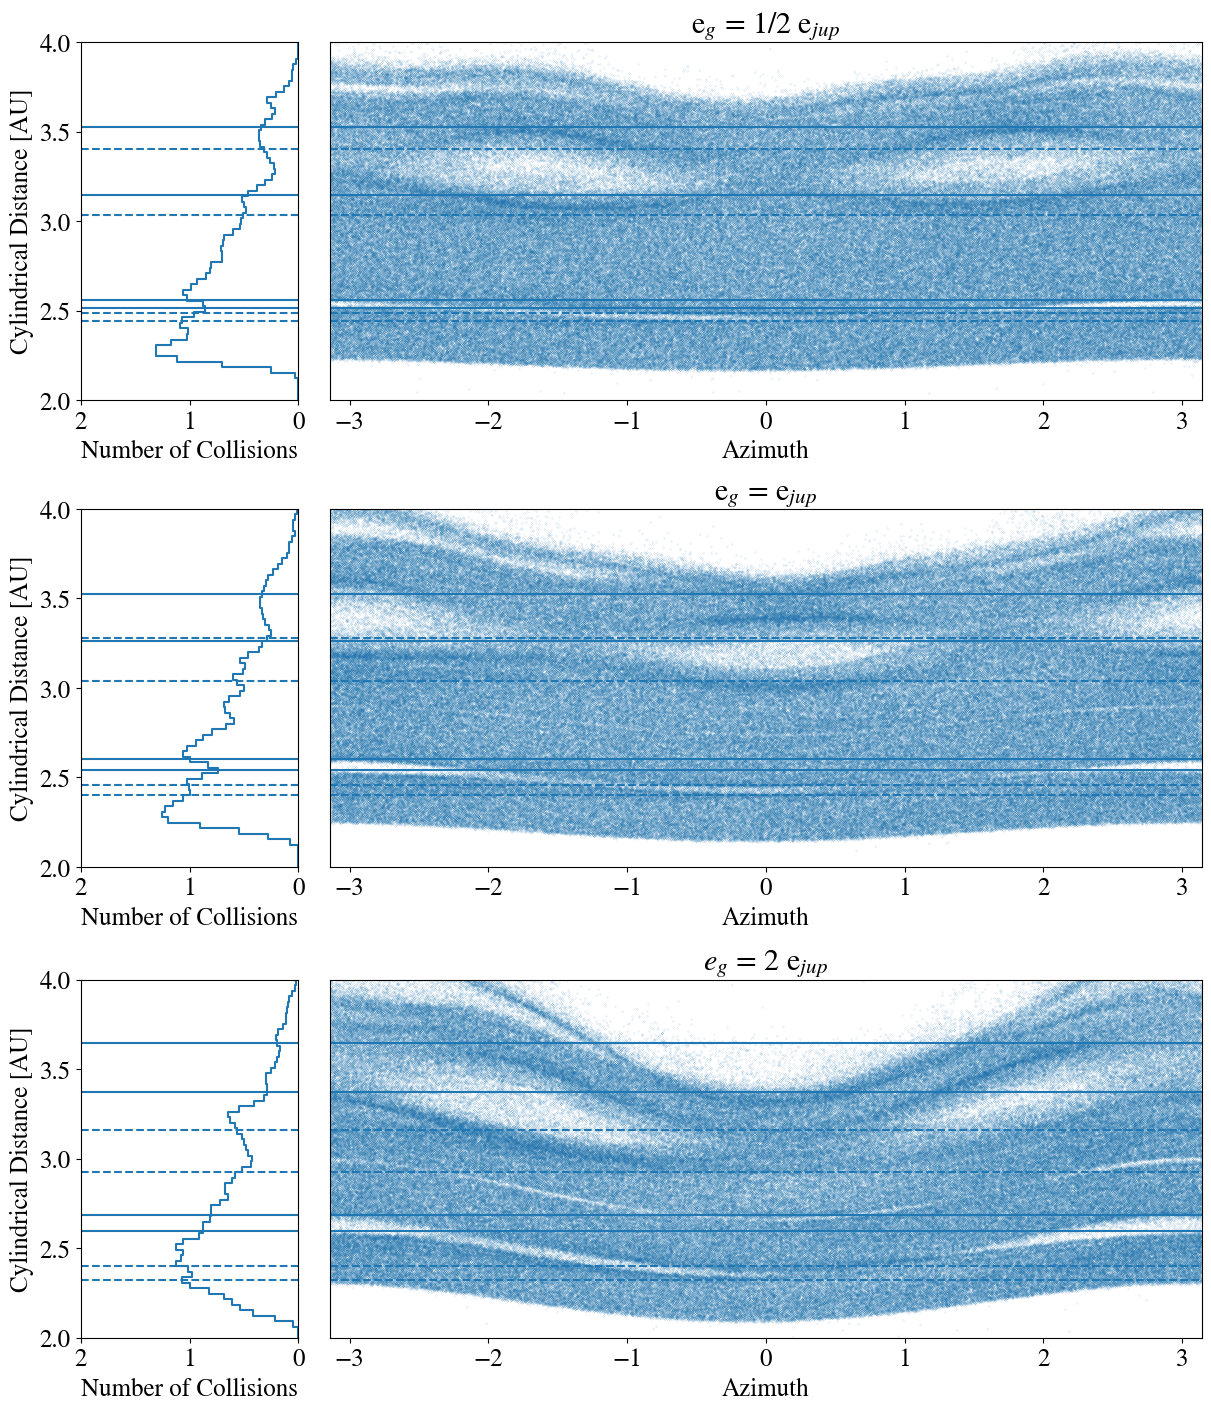
\includegraphics[width=\textwidth]{figures/coll_polar_e.png}
    \caption{The collision profiles in figure \ref{fig:coll_hist_r} are shown alongside the positions of the planetesimals, in polar coordinates. The 
    synthetic dust emission profiles are shown in orange. The dashed and solid lines show the pericenter and apocenter of bodies at the edge of the 
    3:1 and 2:1 MMR. In these figures, the longitude of pericenter of the planet lies at $\theta = 0$ and the present position of the planet is indicated 
    by the vertical line. For the 2:1 resonance, a bump, rather than a dip feature appears when the inner edge or the resonance's apocenter and outer 
    edge's pericenter distance cross. The collision profile near the 3:1 resonance does not appear to follow this same qualitative behavior.
    \label{fig:coll_polar_e}}
\end{figure*}

\begin{figure*}
    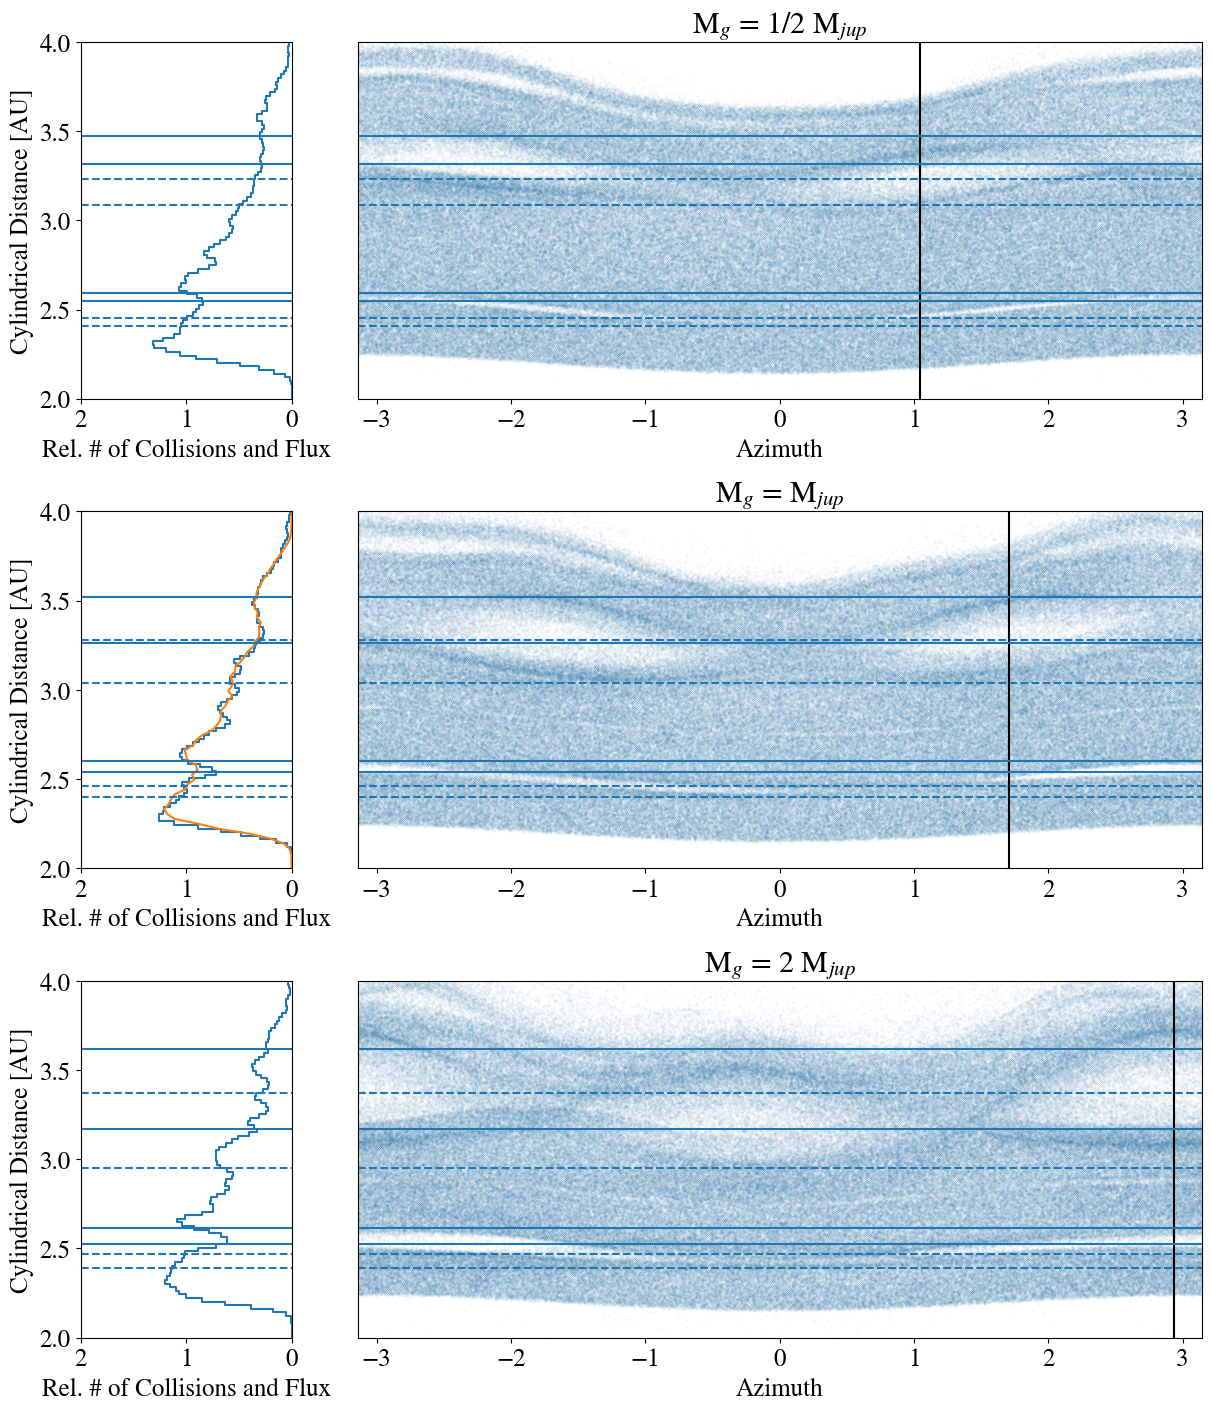
\includegraphics[width=\textwidth]{figures/coll_polar_m.png}
    \caption{Similar to figure \ref{fig:coll_polar_e}, except the eccentricity of the planet is kept constant and the mass is varied.
    This has the effect of changing the width of the resonances, without altering the relative apo or peri distances of
    bodies near the edges. Except for the highest mass case, the apocenter and pericenter distances of the inner and outer edges of the 2:1 
    resonance are too close together to produce much of a dip or a bump feature.\label{fig:coll_polar_m}}
\end{figure*}

\citet{2016ApJ...818..159T} provides a different explanation for this phenomenon. Instead, the nonaxisymmetric structure is claimed to be a product 
of the path that a resonant test particle takes in a frame co-rotating with the planet (see figure 8.4 of \citet{2000ssd..book.....M}). This explanation, 
however, does not hold for a large collection of planetesimals, especially when there is no forced eccentricity. In such a case, the orbits of 
planetesimals near resonance would be randomly aligned, and the axisymmetric structure should become washed out. In the case with a perturbing 
planet planet on a circular orbit, this structure is still present (see figure 3 of \citet{2016ApJ...818..159T}).

With no secular forcing, this dynamical phenomena would produce an underdensity in the radial surface density profile near the center of the 
resonance and an overdensity at each edge in cylindrical distance space. When a forced eccentricity is introduced, the edges of the resonance 
(indicated by the solid and dashed lines in figure \ref{fig:coll_polar_e}), where the pileups are located, begin to explore a wider range of radii over the 
course of a single orbit. If the the aphelion distance of the inner edge becomes comparable to the perihelion distance of the outer edge, the 
overdense regions on each side of the resonance meet and we should expect to see the central dip feature in the collision profile disappear. This is 
exactly what appears to be happening in the middle panel of figure \ref{fig:coll_polar_e}. As the forced eccentricity is increased further, a region 
forms at the center of the resonance where planetesimals from both sides of the resonance spend time (although not simultaneously). When this 
occurs, a bump feature forms in the collision profile near the center of the resonance. This is apparent in the bottom panel of figure 
\ref{fig:coll_polar_e}.

Although the same phenomenon appears to be happening near the 3:1 MMR, the pileups at the edges of the resonance are not as well defined. We 
attribute this to the longer synodic period, compared to the 2:1 MMR. In addition, a number of other nearby resonances, including the 7:2 (at 2.25 
AU), the 10:3 (at 2.33 AU), the 8:3 (at 2.71 AU) and the 5:2 (at 2.82 AU) also likely are contributing to the collision profile in cylindrical distance 
space near the 3:1. The width of the 3:1 MMR is also much narrower than the 2:1, which means that any dip or bump features produced by it would 
require much higher resolution observations. For these reasons, we will focus on the 2:1 MMR as the main diagnostic indicator.

\subsection{Observability of the Dust}

Orange curves in figure \ref{fig:coll_polar_e} show the simulated ALMA flux profiles generated with {\sc CASA} \citep{2007ASPC..376..127M}. Have 
Aaron add in some more text here describing exactly how the profiles were created. Should we add a separate figure to show the flux profiles, or 
include them in figures 6 and 7 like I've started to do here?

\subsection{Varying the Mass}

The dynamical effects of varying the mass of the planet are somewhat simpler, in that doing so does not affect the forced eccentricity of the 
planetesimal disk. Instead, only the width of the resonances changes. The width of a first order resonance scales with $m$ (see equation 
\ref{eq:res_so}), while the leading order terms in the resonant part of the disturbing function, which set the strength of the resonance, also scale as 
$m$. For the 2:1 MMR, the dynamics near the resonance are equally sensitive to changes in eccentricity and mass.

We show the polar structure of the e2m1, e2m2 and e2m3 simulations in figure \ref{fig:coll_polar_m} alongside the radial collision profile. In all three 
cases, the eccentricity of the perturbing planet is set to $e_{jup}$. Changes in the apocenter and pericenter distances of the edges of the 
resonances are entirely due to changes in the libration width here. For the e2m1 and e2m2 simulations, the inner apocenter and outer pericenter 
distances near the 2:1 MMR are quite similar and no strong features appear in the collision profile near this region. For the e2m3 case, the edges of 
the resonances are sufficiently far apart to allow a gap near the center of the 2:1 resonance to appear in the collision profile.

\section{Constraining the Mass and Eccentricity of the Planet}\label{sec:constrain}

\begin{figure}
\begin{center}
    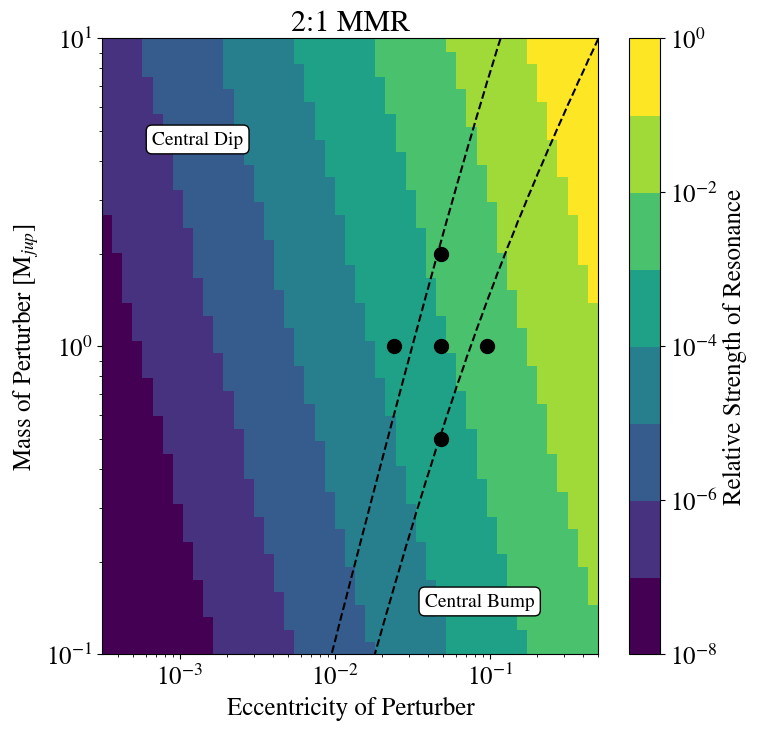
\includegraphics[width=0.5\textwidth]{figures/bump_dip_diag.png}
    \caption{The presence of a dip or bump near the resonances can be used to constrain the mass and eccentricity
    of the perturbing planet. The color scale indicates the relative strength of the features, while the dashed lines
    indicate boundaries in parameter space where a dip or a bump will be produced at the resonance. Combinations of mass and eccentricity that fall 
    between the dashed lines correspond to an inner apocenter and outer pericenter separation at the edges of the resonance that is smaller than the 
    resonance width and therefore will not create any significant feature in the collision profile.\label{fig:bump_dip_diag}}
\end{center}
\end{figure}

The simple 'bump' vs 'dip' structure that we expect to reveal itself in the dust emission from colliding planetesimals in near-resonance with a giant 
planet could potentially be used to place constraints on the mass and eccentricity of the planet. Near the 2:1 MMR, the central dip feature is only 
produced when bodies at the edges of the resonance stay sufficiently separated in cylindrical distance over the course of an orbit. This is achieved 
when either the resonance width is large and the forced eccentricity is small. Conversely, the bump feature is produced when there is a sufficiently 
large amount of overlap between the apocenters and pericenters of the inner and outer edges of the resonance, respectively. This is achieved when 
the resonance is narrow and the forced eccentricity is large.

In figure \ref{fig:bump_dip_diag}, we show the constraints that the presence of a bump or a dip places on the values of $(m_{g}, e_{g})$. A dip is 
produced by sufficiently low eccentricity and high mass planets, while a bump is produced by a low mass or high eccentricity planet. The parameter 
choices for the five simulations presented in the previous section are shown by the black dots. Between the two dashed lines, the overlap between 
the aphelion and perihelion distances of the inner and outer edges of the resonance is smaller than the width of the resonance. In this region, the 
overdense regions on each side of the resonance spend roughly equal amounts of time at all possible cylindrical distances, and no strong feature 
appears in the collision profile.

Because the strength of the 2:1 resonance scales with $e_{g}$ and  $m_{g}$, a sufficiently low mass and low eccentricity planet will not induce 
enough of a perturbation in the planetesimal disk to produce a detectable bump or dip feature. The colored contours in figure \ref{fig:bump_dip_diag} 
indicate the relative strength of the resonance as these quantities are varied. Although the resonance strength is equally sensitive to changes in 
mass and eccentricity, the peri - apocenter overlap of the resonance edges is more sensitive to changes in eccentricity. This is also consistent with 
what was seen in figure \ref{fig:coll_polar_m}, where changing $m_{g}$ by a factor of 4 produced very minimal changes to the resulting dust profile.

In order to actually identify the 2:1 MMR in the dust emission, at least one other resonance must be visible. Assuming the gravitational field in the 
disk is near-Keplerian, the distance ratios between two features can be used to determine period ratios, which can be used to confirm whether the 
features seen are indeed resonances. Although the 3:1 MMR does not appear to follow the simple bump vs dip dichotomy described above, its 
presence should be marginally detectable in all of the cases shown above.

\section{Summary and Conclusions}\label{sec:conclusions}

In this work, we have shown that mean-motion resonances with a perturbing planet produce significant local variations in the collision rate of a 
planetesimal disk. In contrast to \citet{2000Icar..143...45R}, we find that the more prominent interior MMRs, including the 2:1, 3:1 and 5:3, all 
produce structure in the collision profile as a function of semimajor axis. Furthermore, we find that a series of distinctly different features appear 
when collisions are sorted by cylindrical distance from the central star. If enough gas from the protoplanetary disk is still present, dust generated 
from planetesimals collisions will immediately couple to it and fall onto a circular orbit. In this case, the radial dust emission profile, which can be 
observed in the sub-mm, directly traces the radial collision rate and therefore the dynamical activity of the planetesimals.

Near the interior 2:1 MMR, we find that a distinct bump or dip feature is generated in the dust profile. The presence of one of these two structures 
can used to constrain the mass and eccentricity of the perturbing planet. For a high mass, low eccentricity planet, a dip will form in the dust profile 
because the edges of the resonance, where many collisions occur, stay sufficiently separated. If the planet has a low enough mass (which shrinks 
the size of the resonance) or is sufficiently eccentric (which decreases the separation between the apocenter and pericenter distances of the edges 
of the resonance), a bump will instead form. We tested this hypothesis for five different combinations of the planet's mass and eccentricity and found 
that a distinct bump or dip signature is produced as long as the planet properties are sufficiently far from the dividing line in parameter space. This 
diagnostic is more useful for massive, eccentric planets, because the strength of the resonant perturbations scale linearly with both of these 
quantities.

The results presented here appear to be broadly consistent with \citet{2016ApJ...818..159T}, which used collisionless, massless test particles to 
model a planetesimal disk perturbed by a planet. In their case, a dip feature can be seen in the azimuthally averaged surface density profile, 
although they did not test a high enough eccentricity planet in any of their simulations to produce a bump. Another thing to note is that the gap 
morphology seen by \citet{2016ApJ...818..159T} was markedly different for the 2:1 exterior MMR. Whether this would alter the radial collision profile 
for the exterior, rather than the interior 2:1 resonance, is not immediately clear.  Given that the solid surface density diminishes with distance 
($\sim r^{-3/2}$ for the MMSN \citep{1981PThPS..70...35H}), exterior resonances may not be quite as useful for this type of measurement.

Compared to using the gap around the planet as a diagnostic \citep{2013ApJ...777L..31D, 2016ApJ...820...29D}, measuring variations in the dust 
emission near higher order MMRs is much more subtle and requires much higher spatial resolution and sensitivity. As we have shown, the bump vs 
dip feature near the 2:1 MMR is marginally detectable with ALMA for the nearest protoplanetary disks. Another complicating factor is that the inner 
$\sim$ 10 AU of most protoplanetary disks are optically thick in the sub-mm. The solution to this problem is to instead observe in the radio, which 
achieves much poorer resolution. However, future radio facilities like the NG-VLA are expected to achieve sub-AU resolution for nearby planet-
forming disks \citep{2018ASPC..517..147R}. In the more near-term, techniques like Gaussian process fitting present a promising way to recover 
substructure at sub-beam resolution \citep{2020arXiv200507709J}.

\bibliography{references}

\clearpage

\end{document}
